\documentclass[runningheads,a4paper]{llncs}

\usepackage{amssymb}
\setcounter{tocdepth}{3}
\usepackage{graphicx}
\usepackage{amsmath}
\usepackage{verbatim}
\usepackage[margin=1.25in]{geometry}
%\usepackage{amsfonts}
%\usepackage{amsthm}
\usepackage{subfigure}
\usepackage{mathtools}
%\usepackage{caption}
%\usepackage{subcaption}
%\usepackage{cite}
\usepackage{hyperref}
\usepackage{url}
\urlstyle{same}
\newcommand{\keywords}[1]{\par\addvspace\baselineskip
\noindent\keywordname\enspace\ignorespaces#1}

%\makeatletter
%\let\c@lemma=\c@theorem
%\let\c@corollary=\c@theorem
%\let\c@fact=\c@theorem
%\makeatother
%
%\let\realendproof=\endproof
%\def\endproof{\hspace*{\fill}$\Box$\realendproof}
\newtheorem{conj}[theorem]{Conjecture} 
\title{Self Referencing Sequences}
\author{Perry Kleinhenz, Fermi Ma and Erik Waingarten}
\date{}							% Activate to display a given date or no date

\begin{document}

\title{Self Referencing Sequences}
\titlerunning{Self Referencing Sequences}

\author{Perry Kleinhenz \and Fermi Ma \and Erik Waingarten}
%
\authorrunning{Perry Kleinhenz \and Fermi Ma \and Erik Waingarten}
% (feature abused for this document to repeat the title also on left hand pages)

% the affiliations are given next; don't give your e-mail address
% unless you accept that it will be published
\institute{
\protect\url{{pkleinhe, fermima,eaw}@mit.edu}}

\maketitle

\section{Introduction}

\emph{Written by Fermi Ma, edited by Perry Kleinhenz and Erik Waingarten}

We will study a sequences which are self-referencing. That is, each number in the sequence will correspond to a previous number in the same sequence. In particular, we will analyze self-referencing sequences with respect to block lengths. Consider the sequence
\begin{equation}
\label{eq:onetwo}
1,2,2,1,1,2,1,2,2,1,2,2,1,1,2,1,1,2,2,\dots
\end{equation}
We can break up the sequence into contiguous blocks, where each block is a stretch of repeated numbers:
\begin{figure}
\label{fig:sequenceblocks}
\center
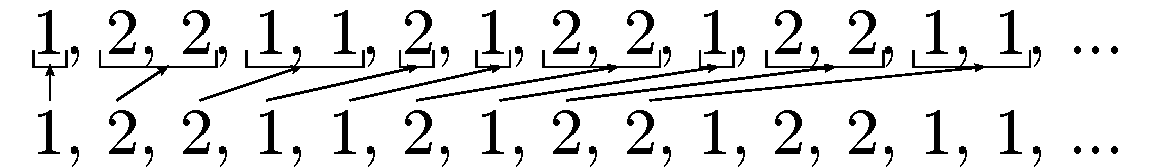
\includegraphics[width=0.5\linewidth]{sequenceBlocks.pdf}
\caption{Sequence broken up into contiguous blocks with lengths generating same sequence.}
\end{figure}

The block lengths, read from left to right, reproduce the original sequence (see Figure~\ref{fig:sequenceblocks}). We call such a sequence \emph{self-referential}. 

Above was an example where the blocks always have elements be either $1$ or $2$. Since we are self-referincing with respect to block lengths, the particular value that the block takes is not as important as the block lengths. Whenever the sequence can only takes two possible numbers, the values of the blocks is unambiguous; the block values simply alternate. As in the sequence above, after a block of 1's, the next block must be a block of 2's and vice versa. However if our sequence was composed of $1$'s, $2'$s and $3'$s there would be ambiguity over which number a new block should begin with. 

For example if the first number is 1, then we could make the second number either a 2, or a 3. In particular, both:
\begin{equation}
1, 3, 3, 3, 2, 2, 2, \dots
\end{equation}
\begin{equation}
1, 2, 2, 1, 1, 3, 1, \dots\\
\end{equation}
are in some sense self-referencing sequences.
Each time we need to specify a new block, we have a choice of two elements. We would like to avoid having a large number of choices in the generation of the sequence, and so we will use the convention that the order in which the elements are presented gives the order they are used in the sequence. 
For example, $(123 )$ will have a order $1 \rightarrow 2 \rightarrow 3 \rightarrow 1$. 

With this rule, the self-referencing sequence generated by $(123)$ that begins with a $1$ is shown in Figure~\ref{fig:onetwothree}.
\begin{figure}
\label{fig:onetwothree}
\center
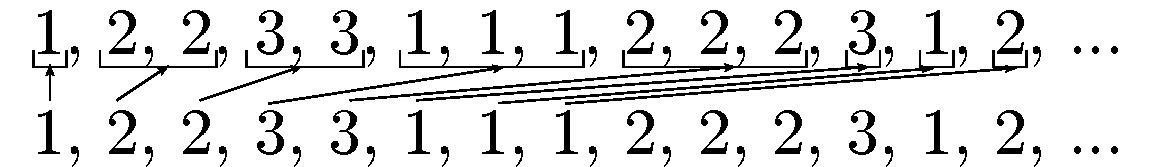
\includegraphics[width=0.5\linewidth]{sequenceBlocks123.pdf}
\caption{Sequence generated by $(123)$ broken up into contiguous blocks.}
\end{figure}

We call the set the sequence is generated over, along with its order the \emph{generating cycle}.

Our main results are:
\begin{itemize}
\item The self-referencing sequence for a given generating cycle is uniquely determined by its first number.
% This doesn't really mean anything... - erik
%
%\item Some characterizations of sequences with the same generating cycle.
\item For some generating cycles there exists an equivalent formulation of self-referencing sequences using substitution rules
\item If a generating cycle has substitution rules then one can compute the limiting density for the numbers in the sequence if a limiting density exists.
\item The limiting densities of the self-referencing sequences of  $(13)$ if such densities exists.
\end{itemize}

In Section~\ref{determinism} we show that if we are given a generating cycle and a starting number for the sequence, the sequence is uniquely determined. In Section~\ref{equivalence}, we consider the limiting behavior of such sequences, and we conjecture that the limiting behavior of a sequence is determined only by the generating cycle, and not the starting number. 

In Section~\ref{iterativeprocess}, we show that there is an alternate way of generating them with an iterative process. In Section~\ref{substitutionrules}, we show how a large number of these sequences can actually be generated with a simple set of substitution rules. We introduce the density problem in Section~\ref{density}, and use ideas developed in Section~\ref{iterativeprocess} and Section~\ref{substitutionrules} to answer the question for certain types of generating cycles. Unfortunately, we find that the open problem of determining the density of the sequences generated by $(12)$ is hard to solve using our methods.

\section{Determinism}
\label{determinism}

\emph{Written by Fermi Ma, edited by Perry Kleinhenz and Erik Waingarten}

We claim that a self-referencing sequence is uniquely determined by the generating cycle $C$ and the starting number $a \in C$. We will prove this by showing that if we are given the first number of the sequence, there is only one way to extend the sequence. In order to do this, we formalize the idea of breaking up a sequence into blocks.

\begin{definition}
A block $B$ is any maximal length subsequence of repeated numbers in a sequence. We denote by $B_i$ the $i$th block of the sequence.
\end{definition}

Here, \emph{maximal length} is a local property that means that the block cannot be extended to include the numbers preceding or succeeding the block, as they will not be the repeated number. Thus, if a sequence $\{a_i\}$ is
\begin{align*}
1,3,3,3,1,1,1,3\dots \,
\end{align*}
the first block is $B_1 = \{1\}$, the second is $B_2 = \{3,3,3\}$, the third is $B_3 = \{1,1,1\}$, and so on. 

Clearly, a sequence can be specified by giving the numbers of the sequence individually, or by specifying all the blocks $B_i$. This is enough to make the following claim:

\begin{proposition}
A self-referencing sequence $\{a_i\}$ is uniquely specified by the generating cycle $C$ and the starting number $a \in C$. In other words, such an $\{a_i\}$ is guaranteed to exist and is unique.
\end{proposition}
\begin{proof} 
The proof is constructive. The self-referential property of the sequence implies that the contents of block $B_i$ are entirely determined by the values of $a$, $i$, and $s_i$. The value of $i$ determines which number is repeated throughout the block. For example, when $i = 1$, the number is the starting number $a$, and when $i = 2$, we use the number following the starting number in $C$, and so on for larger values of $i$. The value of $s_i$ simply dictates the length of block $B_i$.

Thus, the sequence is uniquely given by first ``writing down" $B_1$, followed by $B_2$, followed by $B_3$, etc. One detail is that it remains to check that $s_i$ is known when $B_i$ is written down. However, writing down a block always involves writing down at least one element of the sequence, so the value of $s_i$ is always known when $B_i$ is written down. Note that there is an edge case where $s_i$ is not yet written down if the starting number is 1 and $i =2$. However, in this case, the value of $s_i$ is still known (as it is given by the rule) and thus $B_i$ can still be written down.
\end{proof}
%
%\begin{lemma}
%Let $C$ be a generating cycle. Suppose $\{a_i\}$ and $\{b_i\}$ are both self-referencing sequences with $a_j \neq b_j$ and $j$ is the smallest such number, then $j = 0$.
%\end{lemma}
%
%\begin{proof}
%Suppose $j > 0$, then $a_{j-1} = b_{j-1}$ since $j$ was assumed to be the smallest index where $\{a_i\}$ and $\{b_i\}$ are different. Suppose $a_{j-1} \neq a_j$ and $b_{j-1} \neq b_j$, then we can ask what comes directly after $a_{j-1}$ is the generating cycle; by looking at sequence $\{a_i\}$, we get that $a_j$ comes after $a_{j-1}$, but by looking at the sequence $\{b_i\}$, we get that $b_j$ comes after $a_{j-1}$. This is a contradiction since $a_j \neq b_j$. So lets assume without loss of generality that $a_{j-1} = a_j$, and also, we will assume that $a_{j-1}$ belongs to the $k$th block. Since the sequences are the same up to index $j$, $b_{j-1}$ belongs to the $k$th block. However, this means that $a_k \geq b_k + 1$. So $k \geq j$ and $k$ designates the block length of the block containing $a_j$, and so $k\leq j$, so $k=j$. Figure~\ref{fig:unequalsequences} gives a visual representation of these sequences.
%
%\begin{figure}{hb}
%\label{fig:unequalsequences}
%\center
%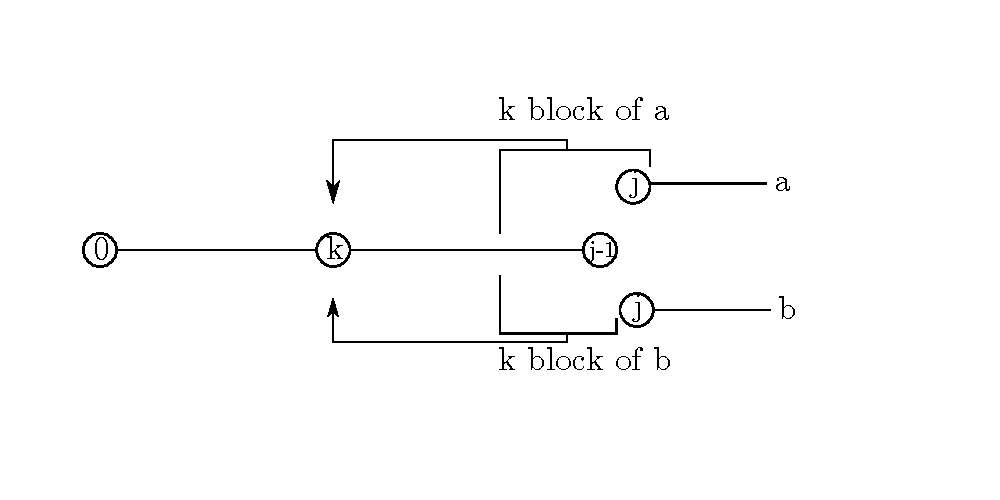
\includegraphics[width=0.5\linewidth]{lemma1.pdf}
%\caption{Self-referencing sequences $a$ and $b$ which differ first at the $j$th element.}
%\end{figure}
%
%This implies that every block before the $k$th block just contains 1's since each block refered it itself. This means that either $j = 2$, or the sequence is not self-referential. But if $j=2$ and $a_1 = b_1 = 1$, then $a_2 \neq b_2$, which means both $a_2$ and $b_2$ comes after $1$ in the generating cycle. 
%\end{proof}
%
%
%
%We present an algorithm that produces the unique self-referencing sequence given a generating cycle and a starting element. Assume the generating cycle is $(a_1 a_2 \dots a_m)$ and that the starting element is some $a_i$. For notational simplicity, if we ever write down $a_k$ where $k > m$, we set this equal to $a_{k (\text{mod } m)}$.
%\begin{quote}
%\textbf{Algorithm:}\\
%Suppose the first number of the sequence is $a_i$. Then the first block of the sequence must be a block of $a_i$ instances of $a_i$, so we extend the sequence to this block. If $a_i$ is not 1, then there is a second element of that block. We read that second element, and then we add a block of $a_i$ instances of $a_{i+1}$ to the end of that sequence. If $a_i$ is equal to 1, we write down $a_{i+1}$ in the second spot, and use the value of $a_{i+1}$ to dictate the length of the second block.\\
%
%This procedure continues deterministically so long as there is an element to read. Every time we write down a block, we read 1 element and write down at least 1 element, thus the end of the sequence will always be at or after the spot we are reading.
%\end{quote}

From this point on, we will denote by $s(C,a)$ the unique sequence with generating cycle $C$ and with starting number $a \in C$.

\section{Equivalence}
\label{equivalence}
\emph{Written by Fermi Ma and Perry Kleinhenz, edited by Erik Waingarten}

In this section, we consider long term equivalence of sequences. We introduce a formal definition of this and establish results that allow us to determine when two sequences are equivalent.  

We would first like to make a formal definition of equivalence. 
\begin{definition}
We say that two sequence $\{a_i\}$ and $\{b_i\}$ are equivalent if there exists some integers $n, k \geq 0$ such that 
\begin{align*}
a_{n+i} = b_{k+i}
\end{align*}
for all positive integers $i$. 
\end{definition}

As an example let us consider sequences generated by $C = (123)$. The sequence which starts with a 2 is 
\begin{align*}
2,2,3,3,1,1,1,2,2,2,3,1,2,3,3,1,1,2,2,3,3,3,\dots \ ,
\end{align*}
and the sequence starting with 3 is 
\begin{align*}
3,3,3,1,1,1,2,2,2,3,1,2,3,3,1,1,2,2,3,3,3,\dots \ .
\end{align*}
If we delete the first two numbers of the sequence starting with 2, and the first number of the sequence starting with 3, we see 
\begin{align*}
2,2,&|3,3,1,1,1,2,2,2,3,1,2,3,3,1,1,2,2,3,3,3,\dots\\
3,&|3,3,1,1,1,2,2,2,3,1,2,3,3,1,1,2,2,3,3,3,\dots \ ,
\end{align*}
that the resultant sequences appear to be identical and thus equivalent. At an intuitive level it seems obvious that these two truncated sequences are identical as they both begin with the same two numbers and the numbers which were removed do not refer to blocks to the right of these numbers.   

In order to formalize and generalize this idea we introduce the notion of a read distance.  
\begin{definition} Consider a sequence $\{a_i\}$. We define the read distance for an index $i$ as the number of terms in between it $a_i$ and the beginning of the $i$th block of numbers.
\end{definition}
The read distance can be any nonnegative integer. For example if we consider the sequence $\{a_i\}$ generated by $C = (1 2 3)$ beginning with a 1  
\begin{align*}
1,2,2,3,3,1,1,1,2,2,2,3,1,2,3,3,1,1,2,2,3,3,3,\dots
\end{align*}
the read distance for $1$ is always $0$ since in a self-referencing sequence, the first number must refer to the first block. The read distance for $2$ is $0$ as the second block of numbers starts at the second number. We can continue to calculate the read distances for this sequence and see that they form a monotonically increasing sequence $0, 0 ,1,2,4,6,6,6,6,7,8,9,\ldots$. 

This monotonicity is true in general, and we can in fact make a stronger statement on the value of the read distance at a given index.
\begin{lemma} 
\label{readdistformula}
Let $\{a_i\}$ be any self referencing sequence generated by some cycle of positive integers. Then the read distance for $i>1$, is 
\begin{equation*}
\sum_{k=1}^{i-1}( a_k - 1)
\end{equation*} 
and the read distance for $1$ is always 0.
\end{lemma}
\begin{proof}
We will prove this using induction. We know that for $i=1$ the read distance is $0$, as the first block always starts at the first number. When $i=2$ the read distance is $a_1-1$. The first block will be of length $a_1$ since the sequence is self referencing, therefore the second block will begin at position $a_1$. The number of elements between position $a_1$ and $2$ is exactly $a_1 -1$.

Now if we assume that our result holds for $i=l$ we would like to show that it holds for $i=l+1$. We know that the distance between the start of the $l$th block and position $l$ is 
\begin{equation*}
\sum_{k=1}^{l-1}( a_k - 1).
\end{equation*} 
This $l$th block has length $a_l$ and so the $l+1$th block will begin $a_l$ positions to the right of the beginning of the $l$th block. Also note that $a_{l+1}$ is one position to the right of $a_l$. Therefore the beginning of the $(l+1)$th block is 
\begin{equation*}
a_l-1 + \sum_{k=1}^{l-1} (a_k-1) = \sum_{k=1}^{l} (a_k-1)
\end{equation*} 
positions to the right of $a_{l+1}$. But this is exactly the reading distance for $a_{l+1}$ and so we have our result.
\end{proof}
Note that because $a_i$ is generated by positive integers we always have $a_k-1\geq 0$ and so the read distance is monotonically increasing. 

%Although this shows us that read distance never decreases it does not tell us how quickly it increases, our next result gives a simple bound on the number of consecutive times the read distance can stay constant. 
%\begin{corollary} Consider a self referencing sequence $\{a_i\}$ generated by $(c_1 c_2 \ldots c_n)$ with $m = \max(c_1, c_2, \ldots, c_n)$. Suppose the read distance for $i$ is $d$, then the read distance for $i+m$ is at least $d+1$. 
%\end{corollary}
%\begin{proof}
%The read distances can stay constant from $i$ to $i+1$ only if there is a $a_{i+1} = 1$. There can be at most $m$ 1's in a contiguous block, so the read distance of $i+m$ is bigger than the read distance of $i$.  
%\end{proof}

Now that we have a nice expression for the value of the read distance at a particular index we can show our first major result which allows us to check only finitely many indices in order to establish that two sequences are equivalent. 
\begin{theorem} 
\label{equivsuff}
Let $\{a_i\}, \{b_i\}$ be two self-referencing sequences generated by the same cycle.If there are integers $m,l$ with the read distance for $a_m$ and $b_l$ are both $d$ and 
\begin{equation*}
a_{m+k} = b_{l+k}
\end{equation*}
where $0 \leq k \leq d-1$ then $\{a_i\}$ and $\{b_i\}$ are equivalent. 
\end{theorem}

\begin{proof}
We will prove this by  induction. In particular we will show for all $k \geq 0$ that $a_{m+k} = b_{l+k}$ and the read distance for $a_{m+k}$ equals the read distance for $b_{l+k}$. By our assumptions we already have this for $0 \leq k \leq d-1$ and so we begin with $k=d$.

Since a new block begins at $a_{m+d}$ and $b_{l+d}$ and $a_{m+d-1} = b_{l+d-1}$ we have $a_{m+d} = b_{l+d}$. Furthermore, by Proposition ~\ref{readdistformula} we have that the read distance for $a_{m+d}$ equals the read distance for $b_{l+d}$. 

Now suppose that  for $k \leq j$ we have $a_{m+k} = b_{l+k}$ and the read distance for $a_{m+k}$ equals the read distance for $b_{l+k}$. We would like to show that this holds for $k = j+1$. By Proposition ~\ref{readdistformula} we actually already know that the read distance for the two is the same, as it is the same for the preceding terms, which are equal.

If $a_{m+k}$ is the last term in a block then $b_{m+k}$ must also be the last term in its block, because the length of blocks is determined by earlier terms which we know to be equal and to have the same read distance. Since $a_{m+k} = b_{l+k}$  in this case we have $a_{m+k+1} = b_{l+k+1}$. 

Otherwise $a_{m+k}$ and $a_{m+k+1}$ are in the same block, and so we only need to show that $b_{l+k}$ and $b_{l+k+1}$ are in the same block as well. But as we argued above the length of blocks is determined by terms earlier in the sequence, which we know to be equal and have the same read distance. Therefore we have $a_{m+k+1} = b_{l+k+1}$ for this case as well. This completes our induction and so $\{a_i\}$ and $\{b_i\}$ are equivalent. 
\end{proof}

This result also allows us to make a general statement for equivalence for sequences that begin with a $1$.
\begin{corollary} If $C = (1 c_1 c_2 \cdots c_n)$, then $s(C, 1)$ and $s(C, c_1)$ are equivalent.
\end{corollary}
\begin{proof}
Let $\{a_i\} = s(C, 1)$ and $\{b_i\} = s(C, c_1)$. The read distance of sequence $\{a_i\}$ for $i=2$ is 0, and the read distance of sequence $\{b_i\}$ for $i = 1$ is 0. In addition, $a_2 = b_1 = c_1$, so by Proposition ~\ref{equivsuff} the two sequences are equivalent.
\end{proof}

We also can demonstrate a sufficient condition for equivalence. 
\begin{theorem}
\label{thm:readfirst}
If two sequences are equivalent then the first element of the shared sequence must have the same read distance in both sequences.
\end{theorem}

\begin{proof}
Assume otherwise. Suppose the two sequences are $\{a_j\}$ and $\{b_j\}$ and we have 
\begin{equation*}
a_{i+l} = b_{i+k} = c_{i}
\end{equation*}
for all $i>1$, such that if $m$ or $l$ were made smaller this relation would not hold. Suppose the read distance for $b_{k+1}$ is $x$ and the read distance for $a_{1+l}$ is $y$. Without loss of generality let us assume that $x>y$ (note that $x \neq y$ as per our assumption).

Since the two read distances are different we know there are two separate blocks of length $c_1$ in the sequence, one which corresponds to $a_{i+l}$ and another which corresponds to $b_{i+k}$. 
Because the two sequences are equal after a certain point and $\{a_j\}$ is self referential there exists some index $n$ such that $c_{n+1}=a_{n+l}$ is the element of $\{a_j\}$ which corresponds to the second block of length $c_1$. 

We now claim that $c_1, c_2, \ldots, c_{n}$  must appear in $\{b_j\}$ such that $b_{i+k-1}=c_{n}$. This is true because $\{b_j\}$ is self referential, and so the length of the blocks of the sequence $\{c_i\}$ must reproduce the terms of $\{b_j\}$. In particular the lengths of the blocks which occur before the second block of length $c_1$ must appear in $\{b_j\}$, and must end right next to the number which refers to the second block of length $c_1$. 

Thus our sequence $\{b_j\}$ is  
\begin{equation*}
\cdots c_1 c_2 c_3 \cdots c_{n} c_1 c_2 \cdots c_n \cdots
\end{equation*}
where the prefix ends at the second $c_1$. We now claim that the common sequence cycles through
\begin{equation*}
c_1 c_2 \cdots c_n.
\end{equation*}
Since the read distance for $b_{1+k}$ is greater than the read distance for $a_{1+l}$, and the sequences are identical for subsequent indices by Lemma ~\ref{readdistformula}, we know that the read distance for $b_{i+k}$ is longer than the read distance for $a_{i+l}$ by exactly $x-y$. Thus $b_{k+i}$ corresponds to the same block as $a_{l+(x-y)+i}$. But $b_{k+i} = c_{i}$ and $a_{l+(x-y)+i}=c_{x-y+i}$ and so $c_{i} = c_{x-y+i}$ and so the common sequence cycles. Because the common sequence cycles and $\{b_j\}$ has the same cycle, but one which begins before the common sequence, $l$ could be made smaller and have the equivalence relation hold. This is contradicts our statement that $l$ is as small as possible. Therefore the first element of the shared sequence must have the same read distance in both sequences. 
\end{proof}

\begin{corollary}
If two self-referencing sequences are equivalent, then their read distance of the shared subsequence is the same everywhere.
\end{corollary}

\begin{proof}
This follows from Theorem~\ref{thm:readfirst} and Lemma~\ref{readdistformula}.
\end{proof}

These conditions for equivalence lead us to make the following conjecture on a sufficient condition for nonequivalence.

\begin{conj} If two sequences $\{a_i\}$ and $\{b_i\}$ are equivalent, then whenever two elements have the same read distances, the two elements are equal. 
\end{conj}

\begin{conj} Any sequence generated by a cycle $C$ is equivalent to any other sequence generated by the same cycle $C$.
\end{conj}

This conjecture is partly motivated by the fact that the property holds for self-referencing sequences from the generating cycle $C= (123)$. For generating cycles with larger numbers, we have been unable to verify or refute the conjecture.. However, in Section~\ref{density}, we show that for some generating cycles the starting number of a sequence does not affect the densities of each number, which provides some evidence for this conjecture.

\section{An Iterative Process}
\label{iterativeprocess}

\emph{Written by Fermi Ma, edited by Perry Kleinhenz and Erik Waingarten}

We change focus in this section and consider how to generate self-referential sequences with an iterative process. We first look at the sequences generated by the cycle $C = (1 2)$.

One possible iterative process is as follows. Let the sequence $s^0$ be 2, and let the sequence $s^{(i)}$ for $i \geq 1$ be the unique sequence that starts with 2 and is such that its block lengths, read from left to right, reproduce the sequence $s^{(i-1)}$. This gives:
\begin{align*}
s^{(0)}&= 2\\
s^{(1)} &= 22\\
s^{(2)} &= 2211\\
s^{(3)}&= 221121\\
s^{(4)} &= 221121221\\
&\vdots
\end{align*}
Let $s^\infty$ be the limit of this process. 
By limit, we mean the limit with respect to each term seperately, so we can define
\[ s^{(i)}_j \rightarrow s^\infty_j \]
as $i \rightarrow \infty$. We claim that $s^\infty$ is the unique self-referential sequence $s(C,2)$. In fact we can prove a more general result about this iterative process.

\begin{theorem}
Let $C$ be some generating cycle. Let $s^0 = a$ for some $a \in C$ where $a \neq 1$, and let $s^{(i)}$ be the sequences generated by the iterative process. Then the limit of this process $s^\infty$ exists and is the sequence $s(C,a)$.
\end{theorem}

\begin{proof}
We prove this by induction on $i$. We show that if $s^{(i)}$ is a prefix of $s(C,a)$, then $s^{(i+1)}$ is a longer prefix of $s(C,a)$. The base case of the induction is satisfied, as $s^{(0)}$ is a prefix of $s(C,a)$.

For the inductive step, we observe that a prefix of the sequence describes the block lengths of a \emph{longer} prefix of the sequence. We know that the sequence it describes is longer because the sequence it describes has length equal to the sum of the original prefix. In other words, the length of $s^{(i+1)}$ equals the sum of of the numbers in $s^{(i)}$, which is strictly greater than the length of $s^{(i)}$ (since there are numbers that are greater than 1). 

The resultant sequence is a prefix of the self referencing sequence because if we apply our process to any prefix of the self referencing sequence it will produce a prefix of the self referencing sequence.  
\end{proof}

Note that we must specify that $a \neq 1$, because that is the only case in which the length of $s^{(i+1)}$ is not strictly greater than the length of $s^{(i)}$. 

It turns out that we can be less restrictive about what our starting sequence, $s^{(0)}$, is. Going back to the case of $C = (1 2)$, we can let $s^{(0)}$ be \emph{any} sequence of 1's and 2's that starts with a 2. And still, the limiting sequence will be the self-referential sequence.
For example, suppose $s^{(0)} = 2,1,1,1,2$. The rules for generating $s^{(i)}$ give:
\begin{align*}
s^{(0)}&= \mathbf{2},1,1,1,2\\
s^{(1)} &= \mathbf{2,2,1},2,1,2,2\\
s^{(2)} &= \mathbf{2,2,1,1,2,1},1,2,1,1,2,2\\
s^{(3)} &= \mathbf{2,2,1,1,2,1,2,2,1,2},1,1,2,1,2,2,1,1\\
&\vdots
\end{align*}
Here, we bold the numbers that form a prefix of $s(C,2)$. We note that $s^\infty = s(C,a)$ because because $s^{(0)}$ contains a 2 at the beginning, which by the above theorem will produce $s(C,a)$ in the limit. We call the rest of each $s^{(i)}$ that is not a prefix of $s(C,2)$ the \emph{tail}.

We now consider two different forms of convergence. We know that $s^{(i)}$ in some sense approaches $s(C,a)$, as arbitrarily many elements at the beginning of the sequence will match up with the beginning of $s(C,a)$ as $i$ increases. However, if the tail of the sequence never entirely disappears, then there does not exist an $i$ where $s^{(i)}$ is exactly a prefix of $s(C,a)$. Thus, we formalize two types of convergence
\begin{definition} We say that a sequence $s^{i}$ is weakly convergent to $s(C,a)$ if $s^\infty = s(C,a)$. We say that the sequence $s^{i}$ is strongly convergent if $s^{(i)}$ is a prefix of $s(C,a)$ for all $i \geq k$ for some $k$.
\end{definition}
It is unclear what conditions must be placed on the starting sequence in order to ensure strong convergence, although based on numerical simulation we make the following conjecture. 

\begin{conj} Let $C = (1,2)$. A sequence $s^{(i)}$ is strongly convergent to $s(C, 2)$ if the starting sequence begins with a $2$ and contains no more than 3 elements. A sequence $s^{(i)}$ is strongly convergent to $s(C, 1)$ if the starting sequence begins with a $1$ and contains between 2 and 3 elements. A sequence $s^{(i)}$ is weakly convergent but not strongly convergent to $s(C, a)$ if the starting sequence begins with an $a \in \{1,2\}$ and contains 4 or more elements.
\end{conj} 
We make this conjecture on the basis on computer simulations which executes the iterative process to at least 20 iterations. More iterations were not completed because after this point the simulations began to take impractically long amounts of time to complete. 

\section{Substitution Rules}
\label{substitutionrules}

\emph{Written by Fermi Ma and Erik Waingarten, edited by Perry Kleinhenz}

The iterative process given in Section~\ref{iterativeprocess} is one way to generate self-referencing sequences. However, for certain generating cycles $C$, there is a simpler ways to perform this iteration using a fixed set of substitution rules. Take $C = (1 3)$ as an example, and consider the sequence that starts with a 3:
\begin{align*}
333111333131333111333\dots
\end{align*}
We can use the iterative process from Section~\ref{iterativeprocess}, and suppose that $s^{(0)} = 33$. We get:
\begin{align*}
\{s^{(0)}\} &= 3,3\\
\{s^{(1)}\} &= 3,3,3,1,1,1\\
\{s^{(2)}\} &= 3,3,3,1,1,1,3,3,3,1,3,1\\
\{s^{(3)}\} &= 3,3,3,1,1,1,3,3,3,1,3,1,3,3,3,1,1,1,3,3,3,1,3,3,3,1\\
&\cdots
\end{align*}
It turns out that we can model this evolution with the following substitution rules:
\begin{align*}
\text{Rule }A: 3,3 &\to 3,3,3,1,1,1 \\
\text{Rule }B: 3,1 &\to 3,3,3,1\\
\text{Rule }C: 1,1 &\to 3,1
\end{align*}
This is to be interpreted as follows. Starting from 3,3, the only possible rule to apply is Rule A, which gives $3,3,3,1,1,1$ at the following iteration. We then apply Rule A to $3,3$, Rule B to $3,1$ and Rule C to $1,1$. Note that at every step, we break up the sequence into chunks of 2 and then simultaneously apply \emph{all} the rules. This will always be possible, since the rules preserve the fact that these sequences have even length. So at the following step, we have 3,3,3,1,1,1,3,3,3,1,3,1, which is $s^{(2)}$. Notice that in general, after the $i$th application of the substitution rules, the sequence is equal to $s^{(i)}$.

Why does this work? Well, first of all, notice that the rules are the natural applications of the self-referential sequence. Also, note that we have decided to make the rules of length 2; if we had made the self-referential rules $1 \rightarrow 1$ and $3 \rightarrow 333$, this would not have worked. In addition, we know that each block length preserves parity. 

We would like to know if we can do this for any generating cycle $C$ and starting number $a$. In particular we would like to be able to simulate our iterative process with substitution rules.

When we apply our substitution rules we should not need to know what happened to blocks other than the one we are currently substituting for. Therefore, each rule must somehow encode the length of  blocks, the number of elements already written in the current block, and what number the current block is composed of. The first condition is simple to implement, as the rules will specify the length of blocks. In order to keep track of the numbers already written, each rule should be self-contained. That is each rule should write complete blocks. In order to comply with the third condition it is enough for the size of the generating cycle to divide the length of the rules. This is so that at the start of each rule, we always know which numbers to write.

Therefore, we can formulate a set of sufficient conditions to make rules to generate the self-referential sequence with generating cycle $C$. 

We want to have a set of rules $R$ where each rule $r \in R$ has length $|r| = l$, such that all $|C|^{l}$ strings are in the rule set and for each $r \in R$
\begin{itemize}
\item each rule writes blocks in the same order of $C$ and each rule has the same starting number
\item $\sum_{i \in r} i$ is divisible by $l$
\item $l$ is divisible by $|C|$
\end{itemize}
Given these conditions on every rule, we can guarantee that the self-referential sequence is generated. Note that in this case, the above example does not satisfy our rules until we say that $1, 3 \to 3, 1, 1, 1$.

Another example, we can have $C = (2 4)$, and we can have that the rules be
\begin{align*}
\text{Rule }A: 2,2 &\to 2, 2, 4, 4 \\
\text{Rule }B: 2,4 &\to 2, 2, 4,4,4,4\\
\text{Rule }C: 4,2 &\to 2,2,2,2,4,4\\
\text{Rule }D: 4,4 &\to 2, 2, 2, 2, 4, 4, 4, 4
\end{align*}

One of the reasons why generating a rule set for $(1 2)$ is complicated is that since $1, ..., 1$ must be in the rule set, the length of the rules must be even (since $|C| = 2$). On the other hand, $2, 1, ..., 1$ must also be in the set and so the rule length must be odd. 

\section{Density}
\label{density}
\emph{Written by Erik Waingarten, edited by Perry Kleinhenz and Fermi Ma}

A topic of interest when considering a self referencing sequence is the relative density of the various elements of the generating cycle. It is unclear if such a density even exists and if so how to compute it for arbitrary generating cycles. In this section, we show how to use substitution rules to compute relative densities for certain sequences if we assume such densities exists. We explain the method and compute the relative density of 3's for $C = (1 3)$. We will also produce bounds on the density of $2$'s $C = (1 2)$ in a way that suggests that the density converges to 2; however, this method is computationally difficult for smaller bounds since the number of cases to check increases exponentially. 

To begin we will discuss a technique that can be used to compute the densities for some generating cycles. In particular, suppose we have a generating cycle $C$ with a set of rules $R$ that satisfy the conditions from the section above. For each rule $r \in R$, we will say denote the rule as $r_l \rightarrow r_r$ as the inputs and the outputs. 

Now we can count the fraction of times $r_r$ appears in the sequence at each step. Since we know the rules, these will become a set of $|R|$ equalities that reference each other. We can take their ratios and solve for the fraction of times that each $r_r$ appears and compute the density by assuming a stable state.

For example, lets look at the rules we have determined for $G = \{ 1, 3 \}$. 
\begin{align*}
\text{Rule }A: 3,3 &\to 3,3,3,1,1,1 \\
\text{Rule }B: 3,1 &\to 3,3,3,1\\
\text{Rule }C: 1,1 &\to 3,1
\end{align*}
Then we can let $3,3,3,1,1,1 = A$, $3,3,3,1 = B$ and $3, 1 = C$. If $A_i$ is the number of occurrences of $A$ in $s^{(i)}$, then 
\[ A_i = B_{i-1} + A_{i-1} \]
Likewise, we have
\[ B_i = A_{i-1} + B_{i-1} + C_{i-1} \]
\[ C_i = A_{i-1} \]
So now we can take the fraction by dividing by the total number of them:
\[ A_i' = \dfrac{B_{i-1}' + A_{i-1}'}{3A_{i-1}' + 2B_{i-1}' + C_{i-1}'} \]
\[ B_i' = \dfrac{A_{i-1}' + B_{i-1}' + C_{i-1}'}{3A_{i-1}' + 2B_{i-1}' + C_{i-1}'} \]
\[ C_i' = \dfrac{A_{i-1}'}{3A_{i-1}' + 2B_{i-1}' + C_{i-1}'} \]
So if we assume a density, there will be a stable state which will be the density, so in the case where $A_i'=A_{i-1}', B_i' = B_{i-1}', C_i'=C_{i-1}'$, we can solve for the fractional appearance of each and get the density of the numbers.

We can compute solutions to this set of quadratic equations and find the density of 3's is approximately $0.602$.

As discussed in the previous section, it is unclear how to establish a set of rules for $C = (1 2)$; however, there is some structure that we can exploit. In particular, we know that the sequences $1, 1, 1$ and $2, 2, 2$ will never appear in the self-referential sequence. This is because such sequences would be part of a block of size at least $3$. 

What does this mean? Well, we know that if there is a density of $1$'s and $2$'s, then that density $d_2$ is bounded between 
\[ \dfrac{1}{3} \leq d_2 \leq \dfrac{2}{3} \]

In general, this gives a procedure for computing the limiting density. For example, now we know that there must be at least one $2$ for every three numbers. So now we can look at how many $2$'s are in any given string of length $9$. We know there must be at least three $2$'s. There are only three cases where there are three 2's in a segment of $9$ numbers in the sequence, namely
\[ 2, 1, 1, 2, 1, 1 ,2 , 1, 1 \]
\[ 1, 2, 1, 1, 2, 1, 1, 2, 1 \]
\[ 1, 1, 2, 1, 1, 2, 1, 1, 2 \]
In each of these cases, we can read the subsequence that must have generated them part of them. In order, they are
\[ 2, 1, 2, 1, 2 \]
\[ 1, 2, 1, 2, 1\]
\[ 2, 1, 2, 1, 2 \]
but each of these are generated by $1, 1, 1$. This means that none of the sequences of length 9 are possible, so in addition to having one 2 for every group of 3, there is another 2 for every group of 9. Therefore, we have shown that the density must be bounded by
\[ \dfrac{1}{3} + \dfrac{1}{9} \leq d_2 \leq 1 - \dfrac{1}{3} - \dfrac{1}{9} \]
In general, we can continue this process, and we did, to show that
\[ \dfrac{1}{3} + \dfrac{1}{9} + \dfrac{1}{27} \leq d_2 \leq 1 - \dfrac{1}{3} - \dfrac{1}{9} - \dfrac{1}{27} \]
Of course, the number of cases to check increases very quickly: there are $3$ choices to put the $2$ in the groups of $3$, $3$ choices to put the 3 groups of 2's and 2 positions within these groups for the groups of 9, and so on. Its not hard to see that this number grows exponentially fast, making it computationally difficult to analyze more cases.

We believe that if there is a way to show this, we will be able to show that the density is $\frac{1}{2}$, since the density will be bounded below by $\sum_{n=1}^\infty \dfrac{1}{3^n} = \frac{1}{2}$ and bounded above by the same number. However, generalizing the procedure to improve the bound seems difficult.

\section{Unresolved Problems}
\emph{Written by Fermi Ma, edited by Perry Kleinhenz and Erik Waingarten}

Our work leaves a number of unresolved problems. 

\begin{itemize}
\item In Section~\ref{equivalence}, we propose the idea that in some sense, the number that we start a sequence with does not matter. In other words, any sequence that uses a certain generating cycle is equivalent to any other sequence created by the same generating cycle.
\item In the same section, we propose a condition for determining when two sequences are not equivalent. We conjecture that if two sequences have unequal numbers with the same read distances, then they are not equivalent. It seems from trying cases that this condition is sufficient, but we have been unable to prove it.
\item In Section~\ref{iterativeprocess} we make a conjecture on when sequences are strongly and weakly convergent. We have not yet been able to investigate strong and weak convergence in great detail, as we have been unable to make precise mathematical statements about these types of convergence. Most of what we know about them comes from analyzing numerical data.
\item In Section~\ref{substitutionrules}, we look at substitution rules for certain ``nice" generating cycles of numbers, such as $(13)$ and $(24)$. These sets allow for substitution rules because they satisfy the trio of properties we outline in that section. However, we do not know that these are the only properties. We leave unresolved the question of determining precisely which sets allow for substitution rules and which ones ones do not. The major difficulty here seems to come in proving that a certain generating cycle does \emph{not} allow for substitution rules.
\item In Section~\ref{density} we were able to compute the density of any sequence with generating cycle $(13)$, and we were able to give bounds on the density of any sequence with generating cycle $(12)$. However, we leave unresolved the question of what the density for $(12)$ actually is, or even if we can obtain tighter bounds.
\end{itemize}

\section{Haikus}
\emph{Written by Fermi Ma}\\

\noindent One, Two, Two, One, One,\\
Two, One, Two, Two, One, Two, Two,\\
One, One, Two, One, One...\\

\noindent For the final draft,\\
we will improve the haikus\\
(and the whole paper).
\end{document}  
